\chapter{Measurement Tools}
\label{chap:Measurement Tools}

\section{Data collection Setup}
\label{sec:Measurement Tools:Data collection Setup}

The data used in the analysis of this thesis, was collected in an unsupervised environment over the course of several days~\ref{sec:data_set}. The experiment involved an APU2E4 access point~\cite{PC_Engines_apu2e4}.

The AP is  equipped with an Atheros~AR9287 wireless chip~\cite{atheros-ar9287}, "The Atheros~AR9287 is a wireless chipset that is compatible with the ath9k Linux kernel driver. It supports IEEE 802.11n wireless networking standards and operates in both the 2.4~GHz and 5~GHz frequency bands. The chipset is known for its reliability, low power consumption, and high throughput. It is commonly used in wireless routers and access points, and it is capable of supporting multiple antennas for improved performance. The ath9k driver provides stable and efficient support for the AR9287~chipset in Linux-based operating systems."

The stations, that were connected to the access point (AP) in the wireless network under observation were a diverse. These stations were located in various positions and orientations, with some being stationary while others were mobile. As the measurements were taken in real-life scenarios, the stationary devices were not static and occasionally moved around, causing variations in signal strength and quality. Mobile devices were moving more frequently, which is observable from signal strength value~\ref{RSSI}.

The movement of the stations may have been caused by the users themselves, as they moved around with their devices, or by other environmental factors, such as interference from other wireless devices or obstacles in the environment. These variations in the signal strength value and quality can impact the transmission rates and the overall performance of the wireless network. Further details will be presented in chapter-3~\ref{chap:Analysis and Optimization}.

Therefore, it is essential to consider the mobility and dynamic nature of the stations when analyzing the wireless network's performance. A detailed description of the environment, including the physical layout and the location of the stations, can provide valuable insights into the performance of the network and help optimize the wireless communication system. Chapter-3 will provide additional information~\ref{chap:Analysis and Optimization}.
The data transmission of each station present on a particular day is depicted in the Figure~\ref{fig:plot_22_population}. For more information on the environment in which the measurements were taken, please refer to the Appendix~\ref{sec:data_set}. 

\begin{landscape}

\begin{figure}[htbp]
  \centering
    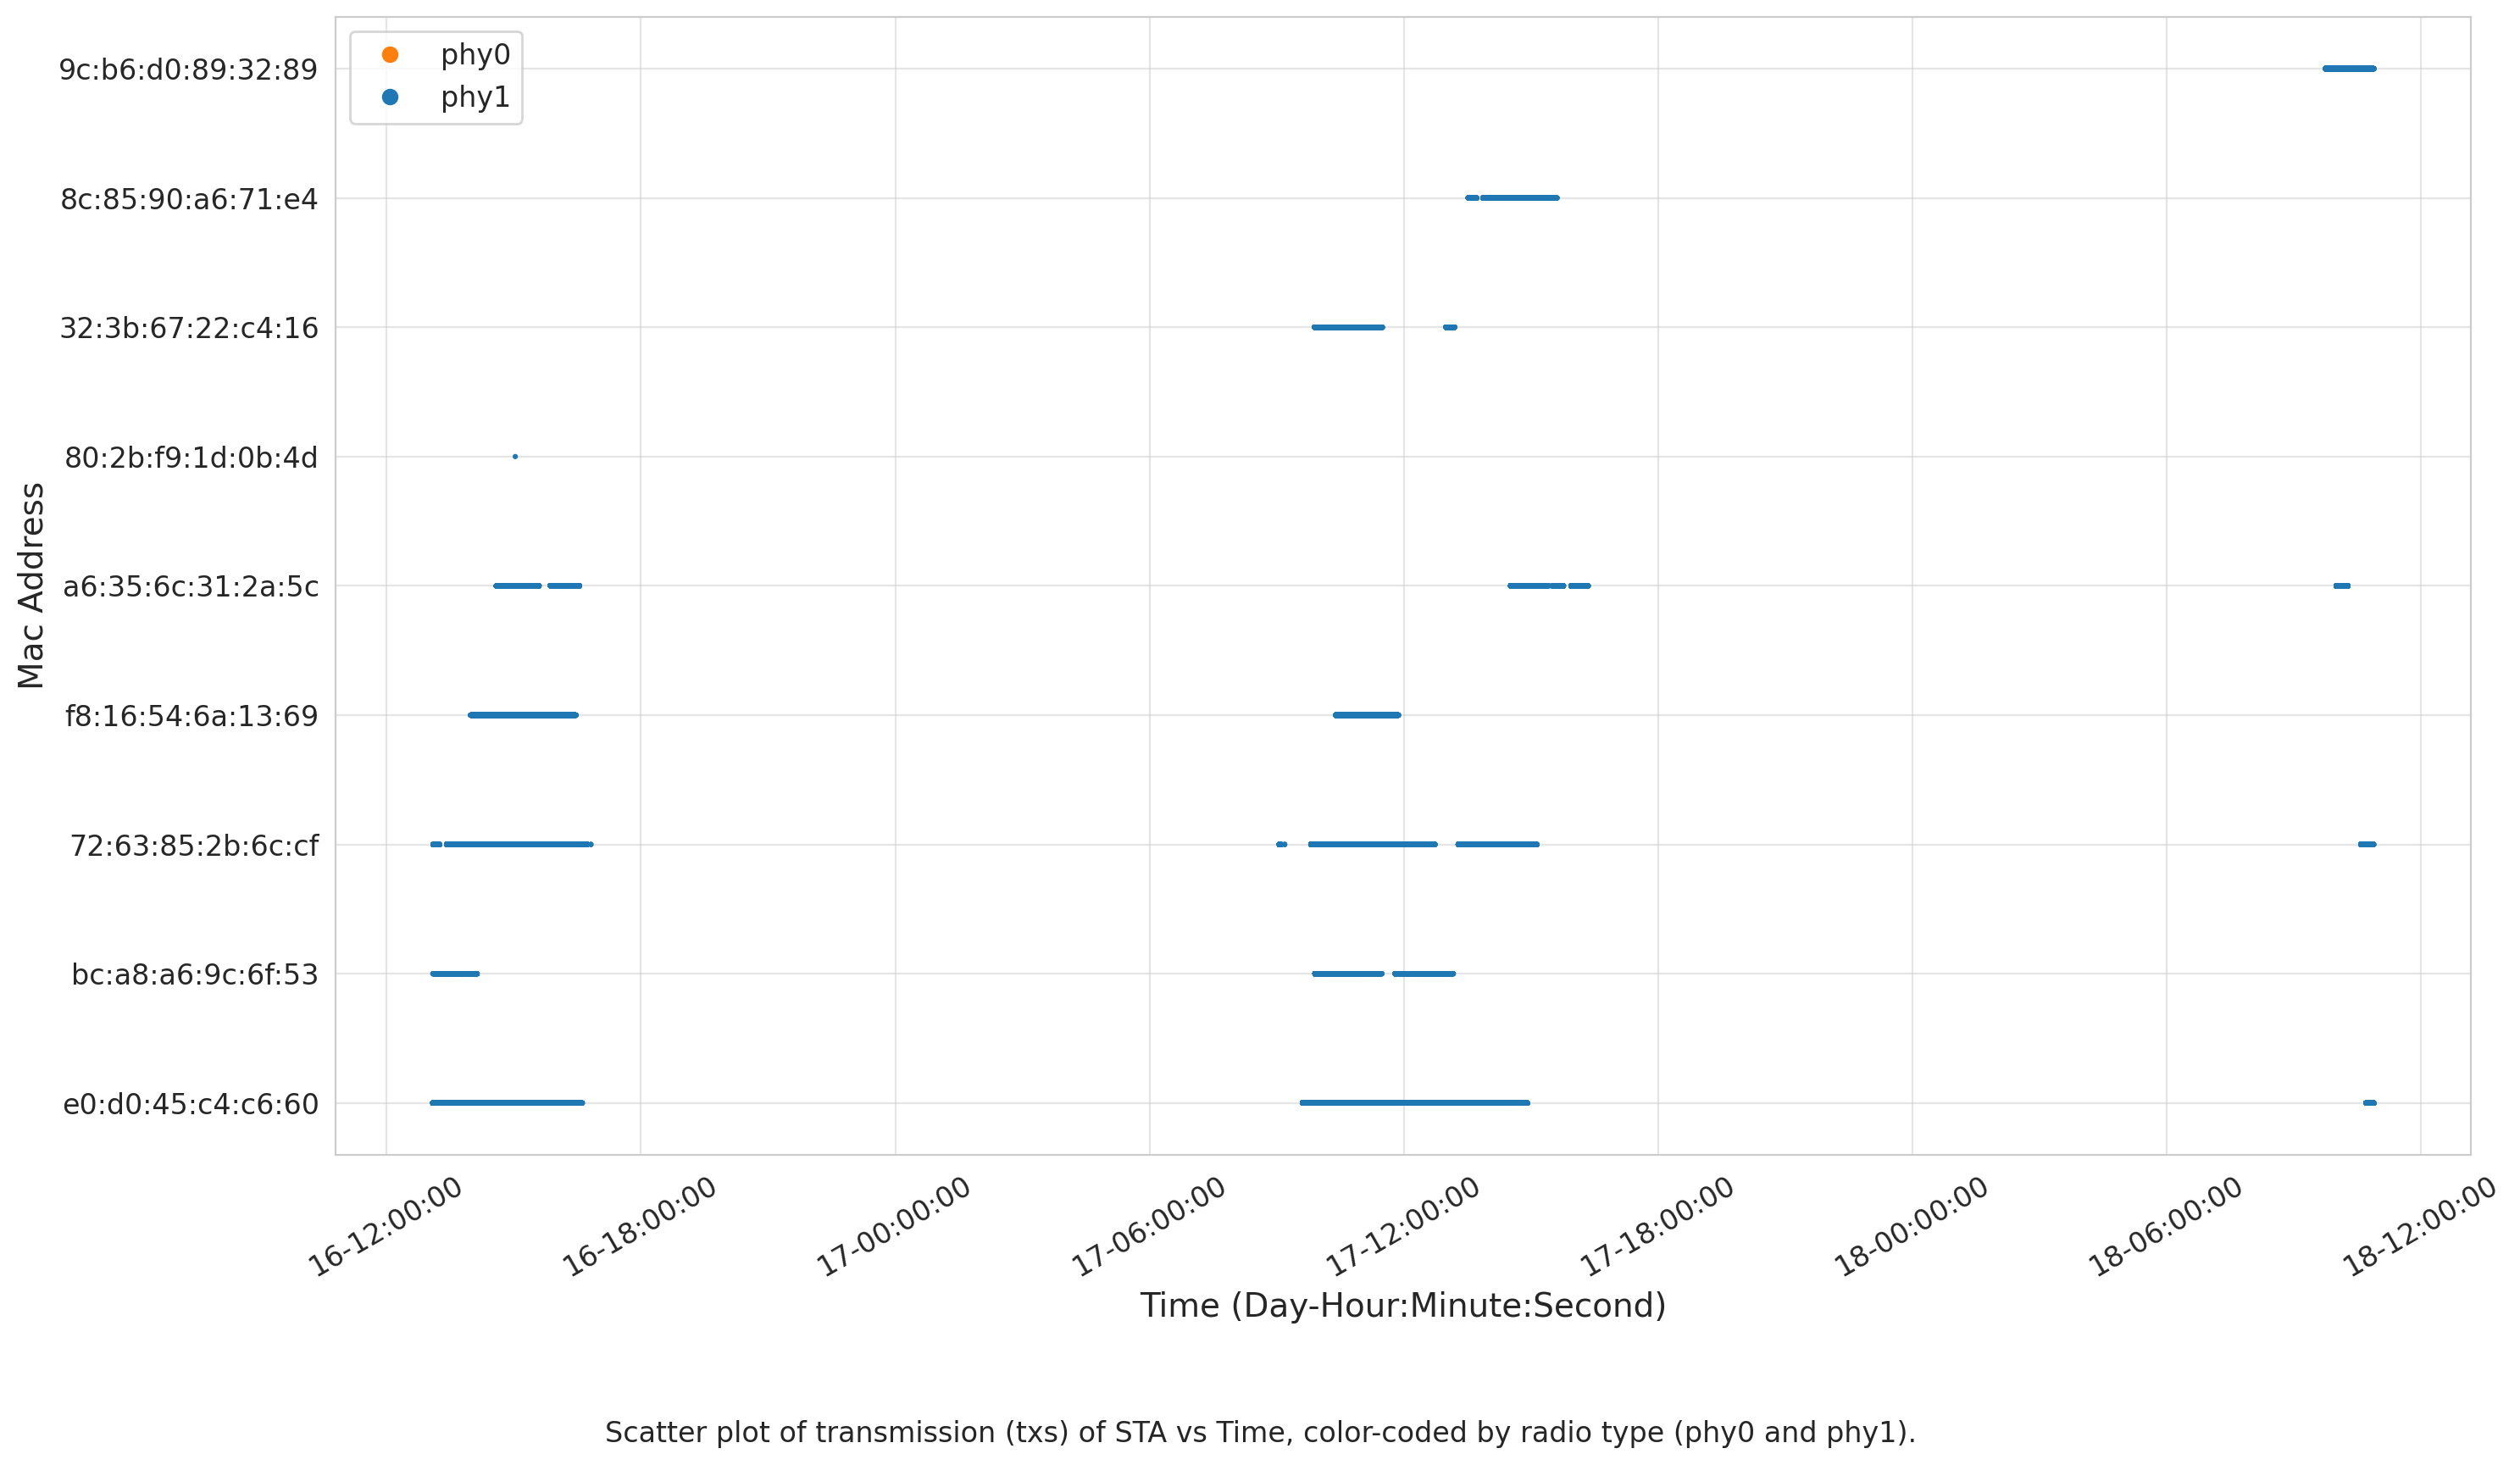
\includegraphics[width=\textwidth, height=\textheight, keepaspectratio]{figures/plots/22.png}
  \caption[Stations' Transmission Over Time]{Scatter plot of transmission (txs) of STA vs Time, color-coded by radio type (phy~0, phy~1, and others).}
  \label{fig:plot_22_population}
\end{figure}
\end{landscape}

\section{Format of Monitoring Information}
\label{sec:Measurement Tools:Format of Monitoring Information}

The trace files fetched from the Linux kernel Minstrel-HT contain detailed information about network events. The first eight lines of a log file serve as the header of a monitoring map for the rest of the event lines. Lines nine through fifty-one are related to groups, and a precise description of these groups is available in reference~\ref{sec:intro:wifiratecontrol:Group creation}. An example of header lines are shown in Figure~\ref{fig:plot_csv1}

After the header lines, each line of the report indicates an event related to a station being connected to the access point, with the MAC address of the station being specified. These events have a nanosecond resolution UNIX timestamp, providing precise information about the exact timing of each event. Figure~\ref{fig:plot_csv2} is a sample of a trace file.

It is important to note that the information contained in these trace files can be used to analyze network performance and identify potential issues. By carefully examining the events recorded in the trace files, researchers can gain valuable insights into the behavior of the network and take steps to optimize its performance.


\begin{figure}[htbp]
  \centering
  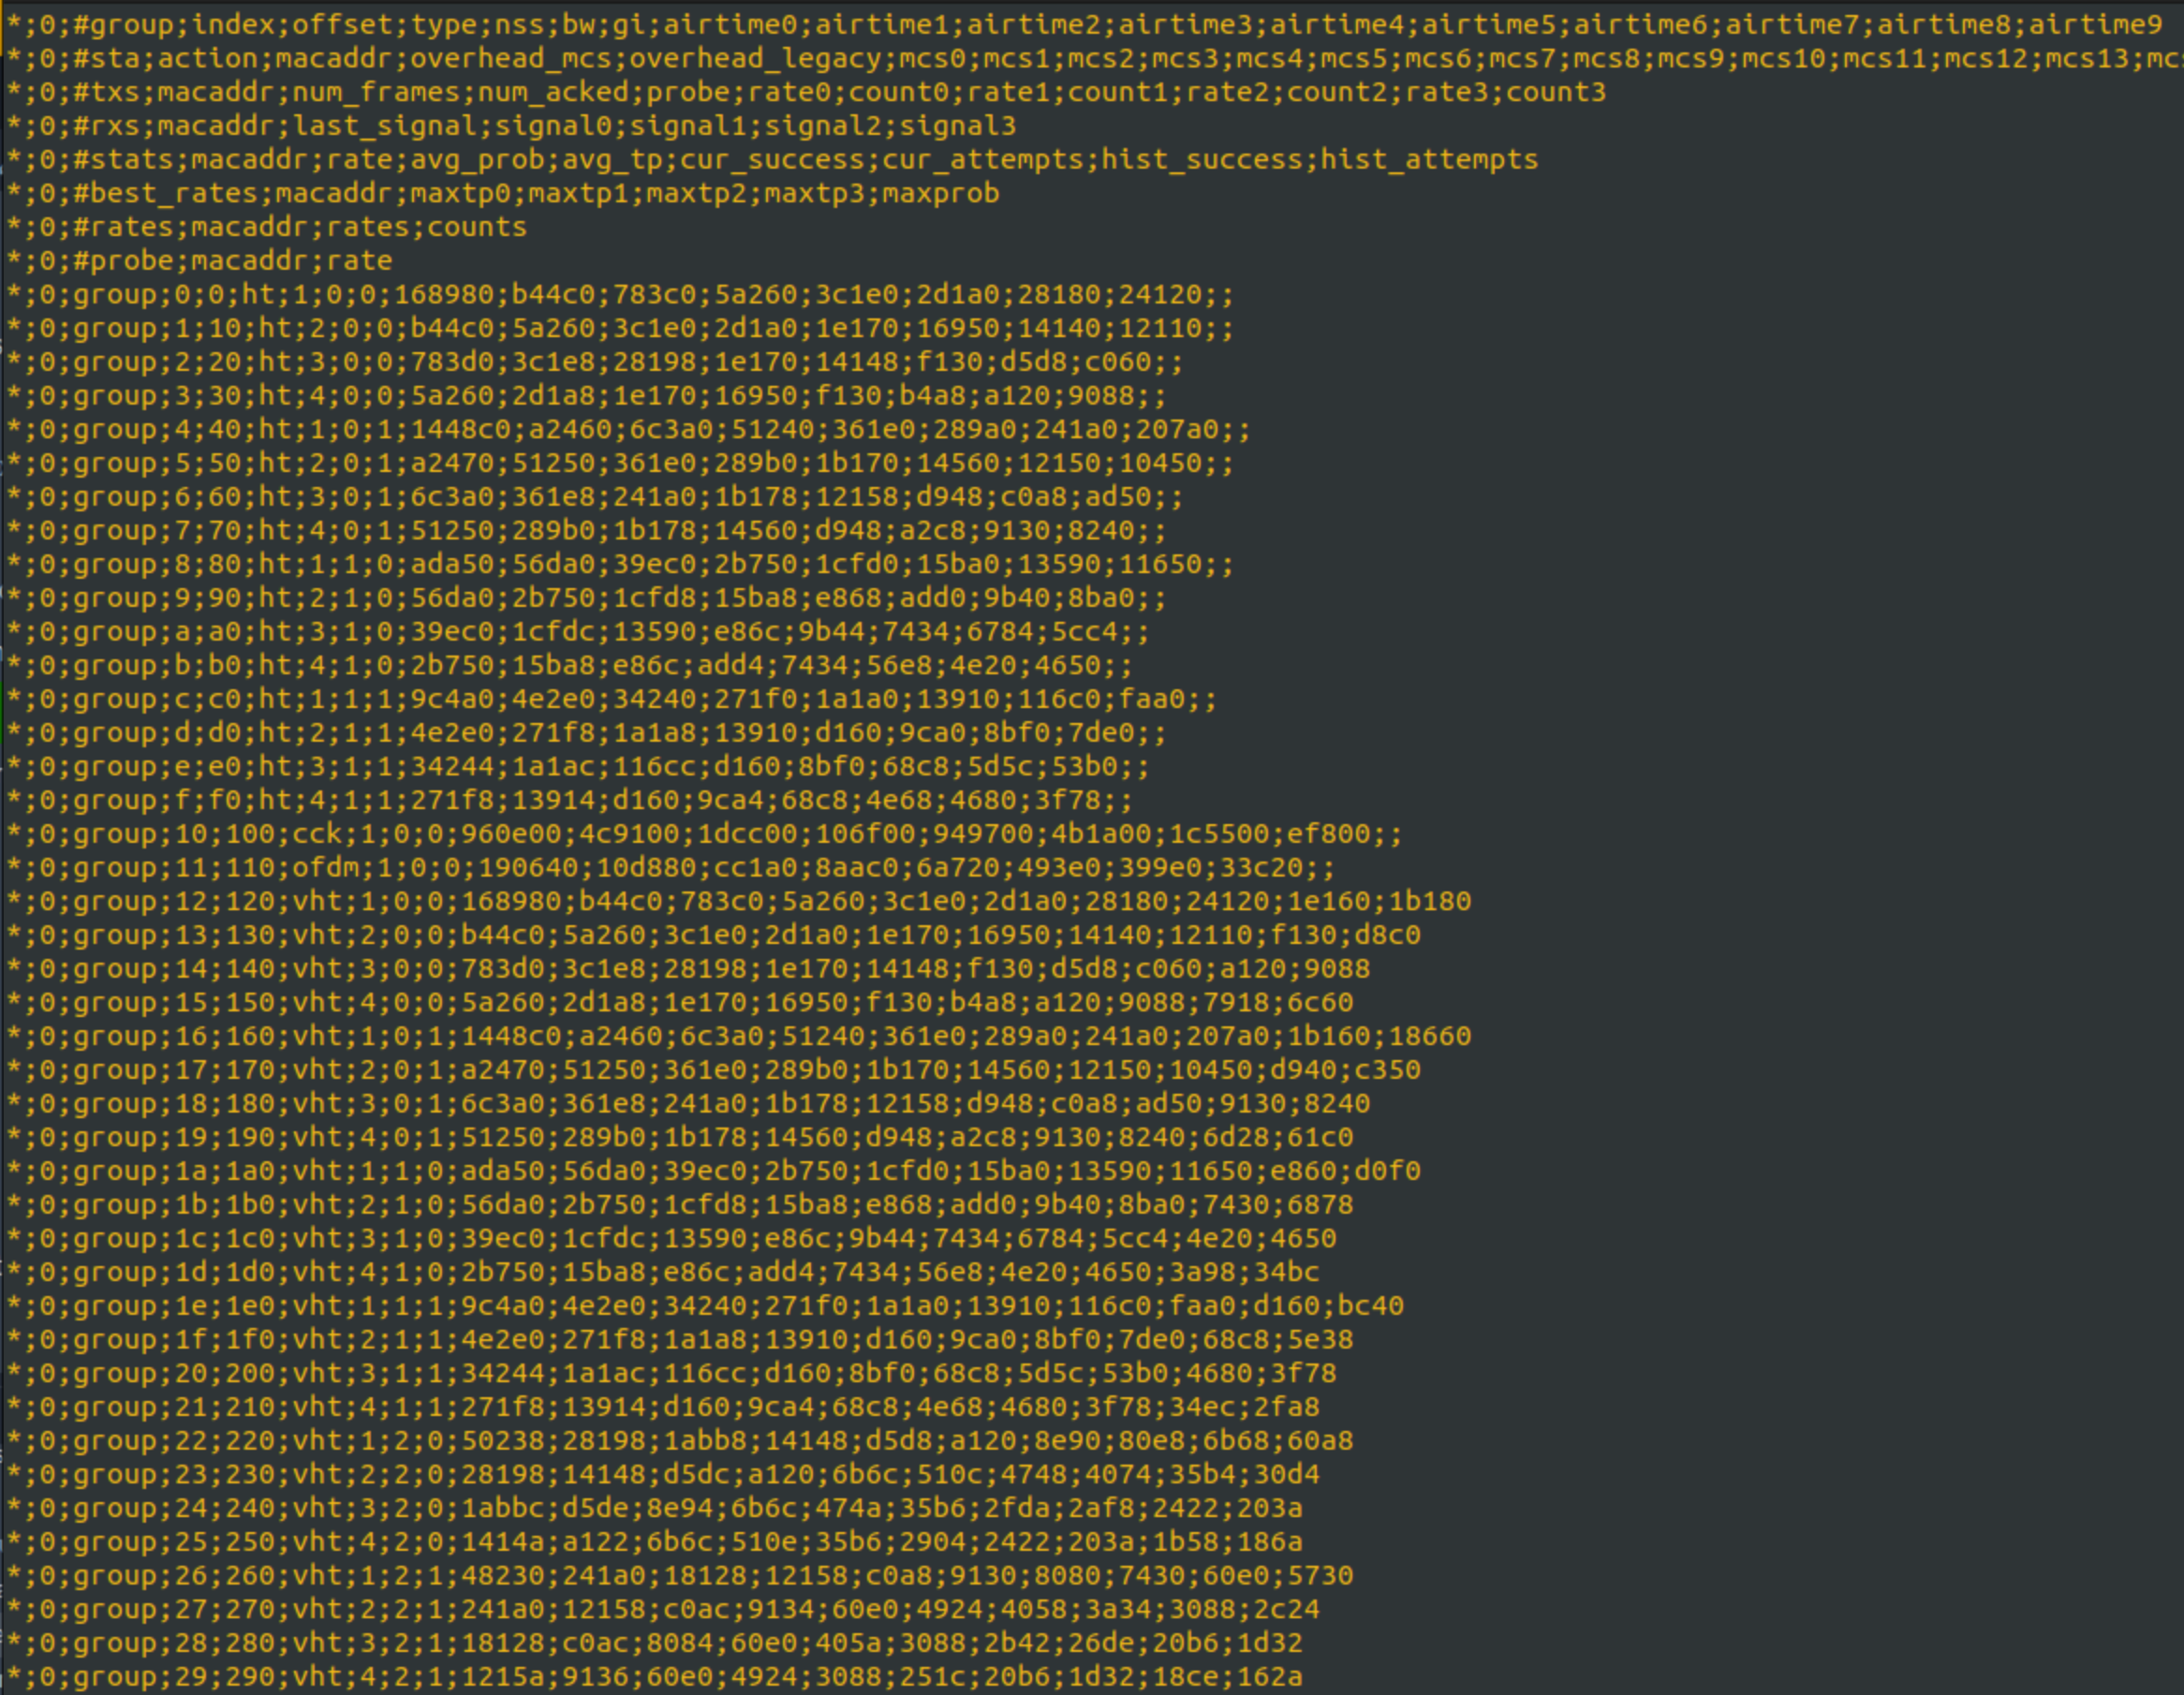
\includegraphics[width=\textwidth]{figures/plots/ratetable.png}
  \caption[Trace File Header]{Here is an example Trace file that contains the header information for GROUP, STA, TXS, RXS, STATS, and best\_rates. It proceeds to give a comprehensive breakdown of the rate specifications for 42 distinct groups.}
  \label{fig:plot_csv1}
\end{figure}

\begin{figure}[htbp]
  \centering
  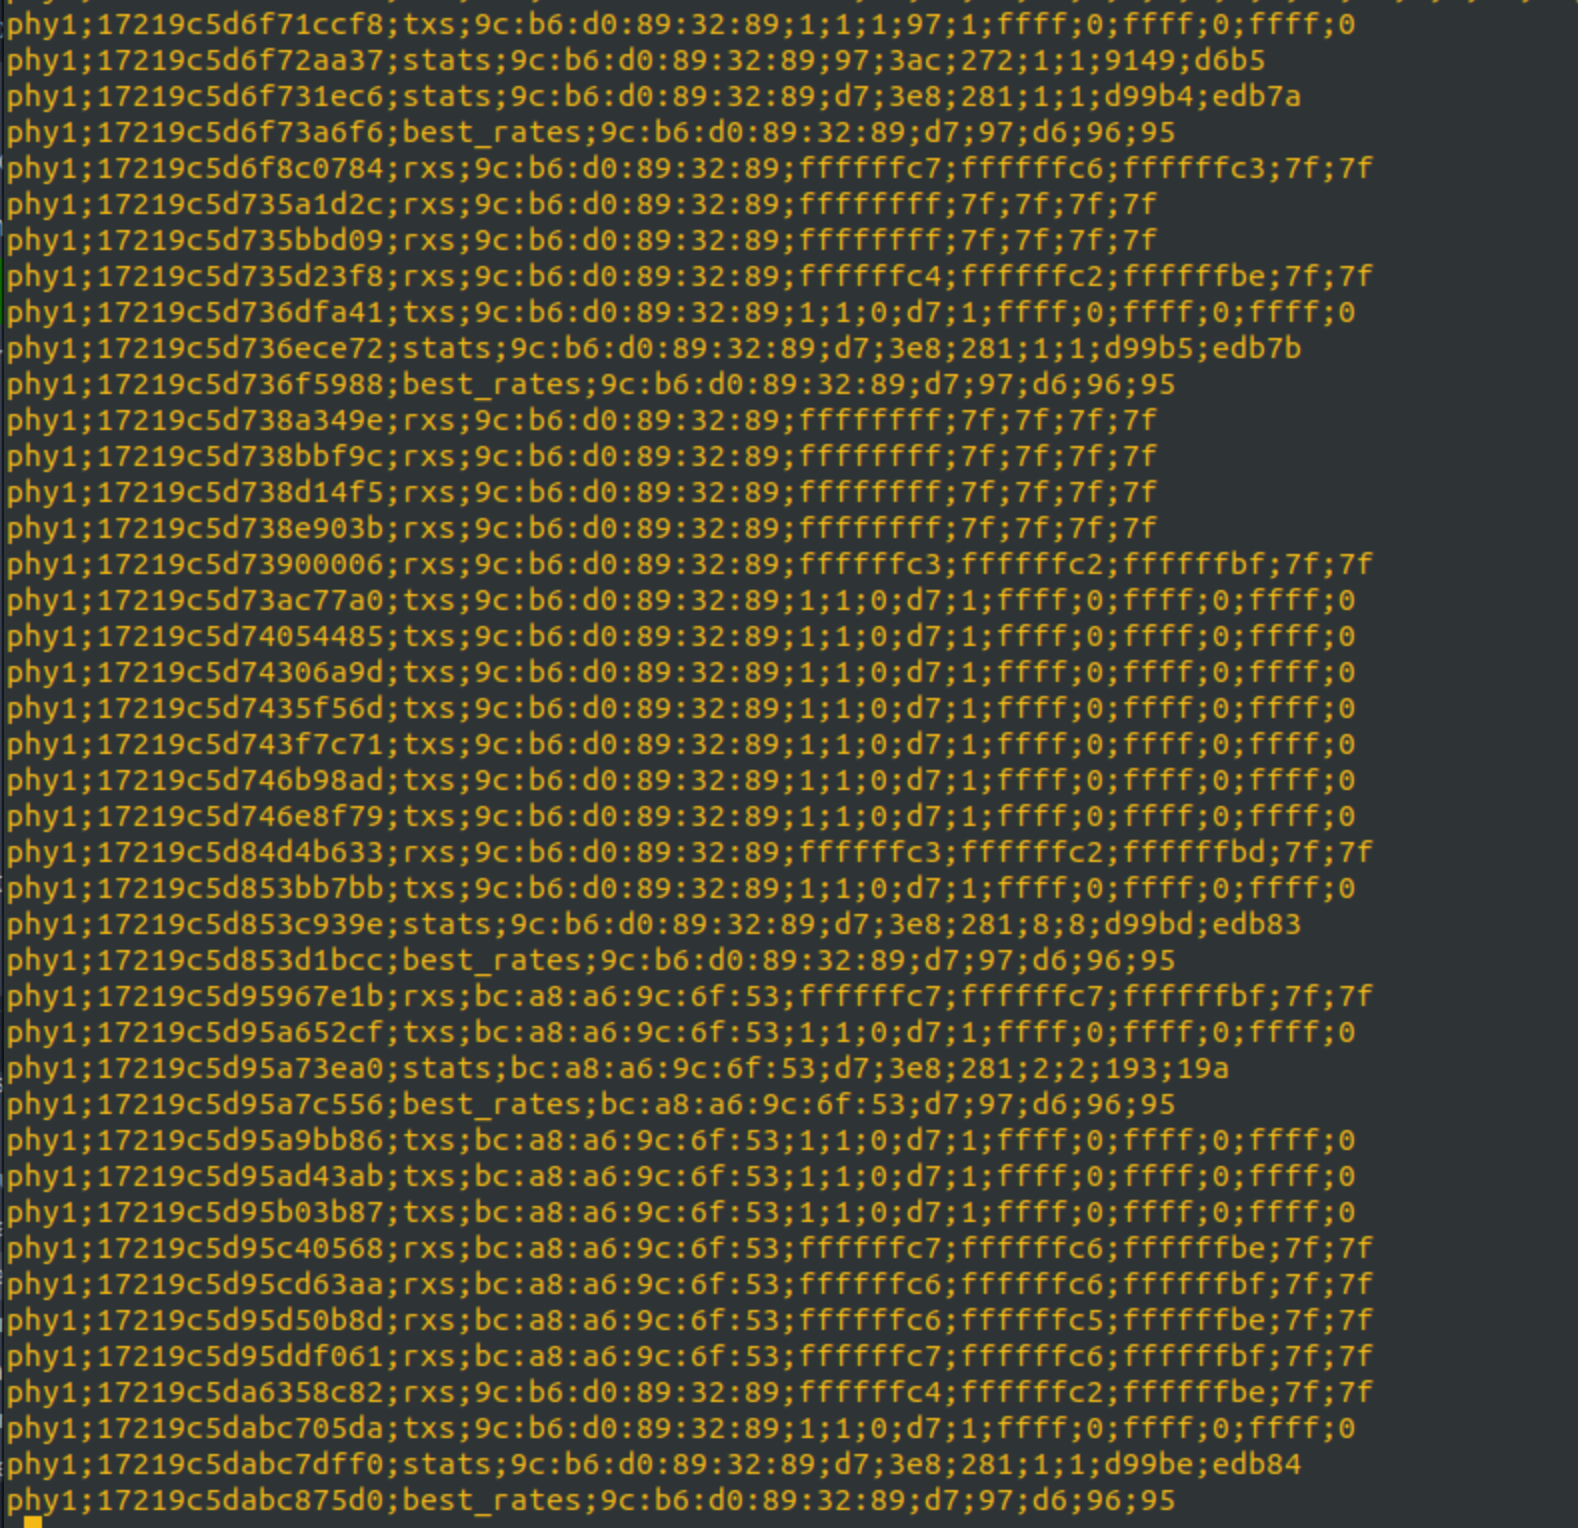
\includegraphics[width=\textwidth]{figures/plots/traceexp.png}
  \caption[Trace File Sample]{Sample of a trace file that contains informative details about transmissions, received signal strength, MAC address of connected stations to AP, and more.}
  \label{fig:plot_csv2}
\end{figure}



\begin{sloppypar}
\begin{itemize}
\item \ GROUP
\begin{lstlisting} [
basicstyle=\small
]
*;0;#group;index;offset;type;nss;bw;gi;airtime*
\end{lstlisting}
Group lines are based on The Modulation Coding Scheme(MCS)index, which has been defined by the WiFi parameters between station and wireless access point.   
    \begin{itemize}
        \item index: Specifies the hexadecimal group index (0-f), (10-1f), (21-29). Group index differs on WiFi parameters such as type, NSS, BW, GI (short guard interval).
        \item offset: Within the group, index (0-7) is being presented. The index number characterizes rates based on airtime values.
        \item type: Very High Throughput (VHT), 802.11ac standard. High Throughput (HT), 802.11n standard. Complementary code keying (CCK) is a modulation that is used by 802.11b (Only used in group 10 - Management frames being transmitted via this modulation). Orthogonal Frequency Division Multiplexing (OFDM) is adopted into 802.11a, 802.11n, 802.11ac standards (group 11 uses this modulation).
        \item nss: Number of antennas used for transmitting (TX)/receiving (RX) been aggregated in NSS (Number of Spatial Stream), which defines how many NSS can be handled by the station.
        \item bw: Bandwidth is represented as 0=20MHz, 1=40MHz, 2=60MHz, 3=180MHz.
        \item gi: Represents short guard interval in Boolean. 0=0.8µs GI, 1=0.4µs GI.
        \item airtime: Corresponds to the offset number of the rate within the group. E.g., rate~21 belongs to group~2, offset~1, airtime~1. Airtime is in nanosecond unit and has been discussed in ~\ref{sec:intro:wifiratecontrol:Group creation}.
    \end{itemize}

\item \ STA
\begin{lstlisting} [basicstyle=\small]
phy*;timestamp;#sta;action;macaddr;overhead_mcs;overhead_legacy;mcs*
\end{lstlisting}
WiFi card standards defines which rate groups are available on stations. STA lines reports this information. Based on "MCS Index,"42 group of MCS rate groups can possibly be available.

    \begin{itemize} 
        \item phy*: Defines the radio interface followed by an index.
        \item timestamp: Timestamp in UNIX nanoseconds.
        \item action: Descriptive information about the action flags presented in~\ref{sta}.
        \item macaddr: MAC address of connected stations.
        \item mcs*: 42~MCS indexes are introduced in the "sta" line. Indexes noted by "ff" indicate the availability of that rate group on the connected station.
        \begin{lstlisting}[basicstyle=\small]
        E.g., phy1;17254b11152721e0;sta;add;bc:a8:a6:9c:6f:53;6c;3c;
        ff;ff;0;0;0;0;0;0;ff;ff;0;0;ff;ff;0;0;0;0;0;0;0;0;
        0;0;0;0;0;0;0;0;0;0;0;0;0;0;0;0;0;0;0;0
        \end{lstlisting}
        A station with the MAC address "bc:a8:a6:9c:6f:53" has been added to the AP list. The groups "0, 1, 8, 9, c, d" contain the available rates on the station. 
    \end{itemize}
    
\item \ TXS
\label{txs}
\begin{lstlisting}[basicstyle=\small]
phy*;timestamp;#txs;macaddr;num_frames;num_acked;probe;rate0;count0..rate3;count3
\end{lstlisting}
Transmission of data frame been reported via TXS lines.

    \begin{itemize}
        \item num\_frames: The number of aggregated data\_frame been transmitted which represented in base16~(hex). It is possible for multiple frame transmissions to be reported in a single line of "txs" within the same timestamp.
        \item num\_acked: The number of sub-frames that have been acknowledged out of aggregated data frames is reported in base16 (hex).
        \item probe: The probe transmission rates are chosen based on the sampling interval of Minstrel HT, which is set at every 20 milliseconds in the current setup. The Boolean flag of the probe defines whether probe transmission rates are enabled or not.
        \item rate *: The chosen rates are presented with "rates*". If the value is "ffff",it shows that no other rate been tried for transmission.
        \item count *: The number of retries for each rate is reported in base16(hex). The maximum retry count per Multi-Rate Retry(MRR)stage is based on standard's protocol as shown in Table~\ref{tab:3a}. The retry attempts continues until possible count, which determines the success or failure of a transmission (It may involves all aggregated sub\_frames or only a part of them).  
        
    \end{itemize}
\begin{table}[ht]
    \centering
    \begin{tabular}{||c c c c||} 
         \hline
         Driver & IEEE 802.11 & mrr stages in hardware & retry count per mrr stage \\ [0.5ex] 
         \hline\hline
         ath5k & b/g/a & 4 & possible to configure/stage \\ 
         \hline
         ath9k & b/g/a/n & 4 & possible to configure/stage \\
         \hline
         mt76 & a/n/ac & 4 & count[0]=1 , count[1,2,3]= fixed up to 15 retries \\
         \hline
         mt76 & b/g/n & 8 & 4 per rate \\
         \hline
         mt76 & b/g/a/n/ac & 8 & 4 per rate \\ [1ex] 
         \hline
    \end{tabular}
    \caption[WiFi Chip Capabilities]{The WiFi Chip Capability table provides information on the number of retry stages and the maximum retry counts for each stage ($count{0}$,$count_{1}$,$count_{2}$,..)  for each driver.}\label{tab:3a}  
  \end{table}  
  
\item \ RXS
\label{rxs}
\begin{lstlisting}[basicstyle=\small]
phy*;timestamp;#rxs;macaddr;last_signal;signal0;signal1;signal2;signal3
\end{lstlisting}
RXS lines are Received Signal Strength values that presents measurement of the power in a received radio signal.

 \begin{itemize}
     \item last-signal: Indicated the power of last radio signal received in specified timestamp.
     \item signal[0..3]: RSSI up to four available antennas. In the rxs function of Minstrel HT algorithm signal is an 32-bit signed integer value represented in hexadecimal notation. To convert it to a decimal value, we first need to extend the sign bit, which is the most significant bit, to fill the remaining bits of the 32-bit value. In this case, the sign bit is 1, which indicates that the value is negative. The value 0x7f is a default signal strength value that is used when an antenna chain is not used to receive a frame. It is a 7-bit signed integer value that corresponds to a signal strength of -1~dBm, which is a relatively weak signal. 
     
 \end{itemize}

\item \ STATS
\begin{lstlisting}[basicstyle=\small]
phy*;timestamp;#stats;macaddr;rate;avg_prob;avg_tp;cur_success;cur_attempts;
hist_success;hist_attempts
\end{lstlisting}
The STATS includes statistics about the performance of a wireless network using the Minstrel HT algorithm.
 \begin{itemize}
     \item rate: This field indicates the transmission rate that is being used by the client device. For each rate been used there is a stats lines presented. 
     \item avg-probe: The average probability of success for transmissions at that rate.
     \item avg-tp: The average throughput achieved by the client device at that rate.
     \item cur-success: The number of successful transmissions at the current rate.
     \item cur-attempts: The number of attempted transmissions at the current rate
     \item hist-success: This field represent the number of successful for the current rate and all previous rates used by the client.
     \item hist-attempts: Defines the number of attempted transmissions for the current rate and all previous rates used by the client.
 \end{itemize}
This information can be used to evaluate the performance of a wireless network and to adjust the transmission rates used by individual station in order to optimize performance.

\item \ BEST\_RATES
\label{bestrates}
\begin{lstlisting}[basicstyle=\small]
phy*;timestamp;#best_rates;macaddr;maxtp0;maxtp1;maxtp2;maxtp3;maxprob
\end{lstlisting}
The "best-rates" lines refer to the best transmission rates for each of the streams available in the wireless device. The $maxtp_{0}$, $maxtp_{1}$, etc. variables represent the maximum throughput achieved for each of the best transmission rates for the respective streams. The $max_{prob}$ value in the output of the algorithm indicates the highest estimated probability of success among all the available rates for a particular client device.

\end{itemize}
\end{sloppypar}

\subsection{Capabilities}
\label{sta}
In Minstrel HT algorithm, to determine the optimal transmission rate for each station based on the current wireless channel conditions, the algorithm maintains a set of data structures that track the past transmissions and their outcomes for each station.
the following commands are used to manage station information via STA lines.
\begin{itemize}
\item \ sta;add  
To add a new station to the algorithm, the "ADD" function is used. When a new station joins the network, the algorithm initializes its data structures with default values and starts collecting data on its transmissions.
\item \ sta;update
After each transmission, the "UPDATE" function updates the data structures for a given STA. The algorithm keeps track of the success or failure of each transmission and updates the relevant data structures accordingly. The updated data is then used to determine the optimal transmission rate for the station for the next transmission.
\item \ sta;remove 
When a station leaves the network, the "REMOVE" function is used to remove its data structures from the algorithm, and its transmissions are no longer considered in the rate control decisions.
\end{itemize}
\newpage





\section{Summary}

The chapter describes the data collection setup and the format of the monitoring information used in the analysis. The experiment involved an Atheros~AR9287 wireless chip, and the stations connected to the AP were diverse and located in various positions and orientations~\ref{sec:Measurement Tools:Data collection Setup}. Then focuses on data trace files fetched from the Linux kernel, and unfurls descriptive details about the headers and all related details present on trace files, such as the definition of each header value, the unit of them and much more~\ref{sec:Measurement Tools:Format of Monitoring Information}.